\chapter{Approach}\label{ch:approach}

The thesis problem statement of developing a profiling framework for seL4 is well defined since we have a comparative tool on Linux in the form of the \texttt{perf\_event\_open} syscall that sets expectations around the desired functionality. However, there is still considerable room for how exactly the profiler should be implemented on seL4. To begin, we will look at some of the limitations of statistical profiling, followed a set of design goals to guide the implementation, and then we will discuss a potential solution.

\section{Statistical Profiling Limitations}

Statistical profiling offers a low overhead approach to profiling, however there are a number of limitations or scenarios where it is not suitable:

\begin{itemize}
    \item When 100\% instruction accurate profiles are required. Due to the latency of the polling interrupts, the address read from the PC may refer to a more recently executed instruction. An illuminating example of this mis-attribution can be seen in a loop where the last instruction is relatively expensive, but the time is attributed to incrementing the loop variable \cite{DocsOProfileInter}.
    \item When the function being profiled is called infrequently. If there are not a sufficient number samples, the profiler may not be able to provide any useful insight into its runtime behaviour.
    \item When no disturbances to the system whatsoever can be tolerated. Sampling requires hardware interrupts to be handled, which may not be suitable for real time applications.
    \item When an interstitial profiling API is required. Due to the nature of sampling, it is imperative that work performed during each profiling interrupt is minimal, to reduce the overhead on the system, and therefore calling user-defined functions during the interrupt handling would not feasible.
\end{itemize}

\section{Design Goals}

\ssp\begin{enumerate}
    \item \textbf{Performance}. The profiler should not impose a significant overhead on the system. Further, the overhead should be directly proportional to the sampling frequency selected by the user.
    \item \textbf{Extensible}. The design should be open for extension, such that new PMU events or configuration options can be added without refactoring the existing codebase. 
    \item \textbf{Portable}. The implementation should not be dependent on any platform and architecture specific details.
    \item \textbf{Configurable}. The design should provide an expressive API to user-space, such that the profiler can be configured to profile specific scenarios. 
    \item \textbf{Verification}. seL4 is a formally verified microkernel and so any extension to the kernel, requires that it be verifiable. While full verification is outside the scope of this thesis, the implementation footprint should be as minimal as possible, and amenable to verification in the future.
\end{enumerate}\dsp

\section{Requirements}

Following on from the design goals, we can now list concrete requirements for the implementation of a profiler for seL4.

\textbf{Requirement 1}. Supports both statistical and event-based profiling.\\
The additional expressivity that arises when supporting both statistical and event-based profiling is evident with the PCL subsystem (see Section \ref{sect:pcl}), as it allows the user to configure sampling based on (microarchitecture) events. This means that users are not constrained to only sampling based on CPU cycles.

\textbf{Requirement 2}. Supports non-destructive profiling.\\
The term \textit{non-destructive} refers to a type of profiling which does not require the program to be recompiled in order to be profiled. 

\textbf{Requirement 3}. Symbol resolution.\\
The profiler should resolve raw addresses, obtained as part of the sample, to their corresponding symbol, as it is critical to the usability of the tool. This includes resolving symbols for the kernel, shared libraries, and user-space programs.

\textbf{Requirement 4}. Supports system-wide profiling.\\
The ability to monitor the whole system allows mode switches between kernel-mode and user-mode to be observed. To profile IPC for example, requires system-wide profiling be supported. 

\textbf{Requirement 5}. Transport independent.\\
Unlike the \texttt{perf} utility on Linux, we cannot assume a filesystem will be present to write the profile data to disk. Therefore, where the profile data is written should be provided by the user. This decouples the responsibility of collecting the data from storing the data.

\textbf{Requirement 6}. Addresses lockstep sampling.\\
Lockstep sampling occurs when the profiling samples occur at the same frequency as a loop in the program. The result is that each sample is taken at a similar location in the loop, therefore giving the appearance that it is the most common operation, and possibly a performance bottleneck.

\textbf{Requirement 7}. Interoperability with \shellcmd{perf report}.\\
We should not reinvent the wheel, but instead look to leverage the existing ecosystem of tooling built around the PCL subsystem. 

\section{Targeted Platform}

All major platforms support performance monitoring (see Section \ref{sect:platform_support}). The interface for accessing the PMU counters differs on each platform. While libsel4bench (see Section \ref{sect:libsel4bench}) defines an interface for accessing and configuring the PMU counters \cite{github_libsel4bench_sel4bench_header} which abstracts over platform specifics, to begin we want to focus on a single platform or architecture. Considering that ARM is the most supported platform on seL4 \cite{DocsSeL4Hardware}, we should start with ARM, and in particular ARMv8-A (A refers to the A-profile, which is targeted towards operating systems).

\section{Design}

At a conceptual level, the PCL subsystem is a suitable reference approach for abstracting over the PMU counters. It is also an example of a working implementation. However, there are a number of implementation specific details that limit its usefulness in the context of seL4:

\ssp\begin{itemize}
    \item \textbf{Requires a filesystem}. The \shellcmd{perf record} command assumes that the output will be written to a file. There is no requirement for an seL4 system to have a mounted filesystem, and therefore we cannot make this assumption. However, the \texttt{perf\_event\_open} Linux syscall (see Section \ref{sect:perf_event_open}) writes sample data to a shared memory, which is also possible on seL4.
    \item \textbf{Inherit complexity}. Linux is deployed everywhere, and therefore the PCL subsystem was designed and built to support all possible uses cases, since it could not predict how users might want to use the subsystem. For seL4, we can limit the inherit complexity by focusing only on the use cases relevant to seL4 users.
    \item \textbf{Interrupt handling}. The PCL subsystem will handle the interrupt and generate a sample within the kernel itself. For seL4, there is no evidence that this needs to be happen with the kernel, and therefore should be moved to userspace. As a consequence, the shared ring-buffer between the user thread and the kernel is not required for seL4.
    \item \textbf{POSIX/Linux APIs}. The PCL subsystem depends on either POSIX or Linux specific APIs. seL4 does not implement a POSIX/UNIX like interface and therefore either syscalls in the PCL subsystem need to be mapped to corresponding syscalls in seL4, or another approach needs to be devised where no mapping exists.
\end{itemize}\dsp

Thus, our proposed design looks to borrow concepts from PLC where possible, but is congruent with an seL4 environment. The design is comprised of the following components:

\ssp\begin{itemize}
    \item \textit{Profiling server} is responsible for configuring the PMU counters, handling interrupts from the PMU and generating samples. If a thread wants to start or stop profiling, it does so by sending a request to the profiling server.
    \item \textit{Sample ring-buffer} is a ring-buffer that stores the sample generated during each PMU interrupt.
    \item \textit{Debug seL4 kernel} is required since on ARM, user-mode access to PMU counters must be enabled in kernel-mode. Note, there already exists the ability to compile a debug version of seL4.
\end{itemize}\dsp

When the ring-buffer within the profiling server reaches capacity, the buffer needs to be flushed. The server does not make any assumptions as to where the data in the buffer should be written, and instead invokes a capability supplied from the requesting thread to flush the buffer. To help illustrate how this would work in practice, we will walk through a scenario where the profiler is running on an embedded device, and the profile data is being sent to a Linux machine via the network (Figure \ref{fig:profiler_design}). 

\begin{figure}[!h]
    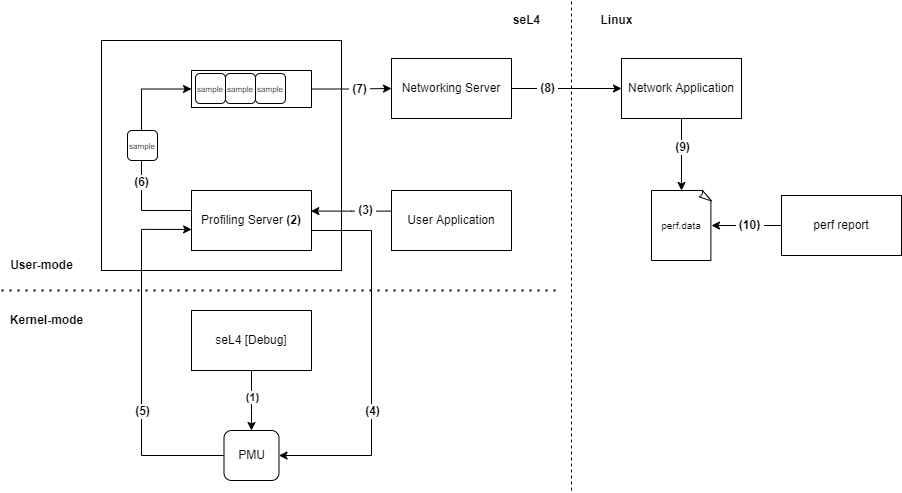
\includegraphics[width=\linewidth]{thesis_a_design_overview.drawio}
    \caption{Design overview for a profiler in seL4, where the transport layer been configured such that measurement data is sent via the network and stored on the receiving Linux machine.}
    \label{fig:profiler_design}
\end{figure}

\ssp\begin{enumerate}
    \item The debug seL4 kernel enables user-mode access to the PMU counters.
    \item The profiling server is provided a capability in order to service interrupts from the PMU.
    \item The user application that would like to start profiling sends a request to the server (via IPC).
    \item The profiling server then configures the PMU via MSRs (see Section \ref{sect:programming_pmu}).
    \item Once the PMU counter overflows, it sends an interrupt, which is ultimately handled by the profiling server.
    \item The profiling server reads the appropriate PMU counter and generates a sample which is stored in the ring-buffer.
    \item When the ring-buffer reaches capacity, the capability provided by the user application was a capability to send a packet via the networking server. The profiling server then invokes the capability, which results in the samples in the buffer being transferred across the network.
    \item A network application on the Linux machine receives the profile data, which conforms to the perf file format (see Section \ref{sect:perf_file_format}), and is written out to a file on disk.
    \item Lastly, the \shellcmd{perf record} command on Linux is used at a later stage to display the profile data.
\end{enumerate}\dsp